\documentclass[
    12pt,
    a4paper,
    brazil,
    english
]{article}
\usepackage{algorithm}
\usepackage{algpseudocode}
\usepackage{titlesec}
\usepackage{amssymb}
\usepackage{graphicx} % For including graphics (e.g., logos)
\usepackage{float} % To place floats (e.g., algorithms) precisely
\usepackage{ragged2e} % For text justification
\usepackage{caption} % To control caption formatting
\usepackage{amsmath} % For better text formatting in math mode

% Document metadata
\title{Lista Avaliativa 3}
\author{Pedro Brasil Barroso - RA 260637}
\date{\today} % Automatically inserts today's date

%\captionsetup[algorithm]{labelformat=empty} % Removes numbering from algorithm captions
\renewcommand{\thealgorithm}{} % Removes the numbering but keeps Algoritmo
\setlength{\parindent}{1.5em} % Adjust the 1.5em to control the size of the indentation


\begin{document}

% Custom title page
\begin{titlepage}
    \centering

    % Insert a logo if you want
    %\includegraphics[width=0.2\textwidth]{logo.png} % Replace with your logo's path
    \vspace*{6cm}

    {\LARGE \textbf{MC558 - Lista Avaliativa 3}}
    
    \vspace{5.5cm}
    {\Large Pedro Brasil Barroso - RA 260637}

    \vfill

    {\Large Universidade Estadual de Campinas} \\ % Replace with your university name
    {\Large Instituto de Computação} \\

    \vspace{1cm}
\end{titlepage}

\textbf{Problema selecionado:} 7 - \textit{Fábrica de sorvetes}

\vspace{0.5cm}

\textbf{(a) Apresente o programa linear explicando as variáveis, função objetivo e restrições.}

\vspace{0.5cm}

\textbf{Variáveis:}

\begin{itemize}
    \item $x_c$: quantidade de sorvete de chocolate (em litros) a ser produzida.
    \item $x_b$: quantidade de sorvete de baunilha (em litros) a ser produzida.
    \item $x_m$: quantidade de sorvete de morango (em litros) a ser produzida.
\end{itemize}

\textbf{Função objetivo:} maximizar o lucro total obtido com a venda dos sorvetes.

\textbf{Restrições:} Cada tipo de sorvete requer uma quantidade específica de leite, açúcar e saborizantes para ser produzido. Além disso, há uma quantidade limitada desses ingredientes disponíveis e uma quantidade mínima de cada tipo de sorvete que deve ser produzida:

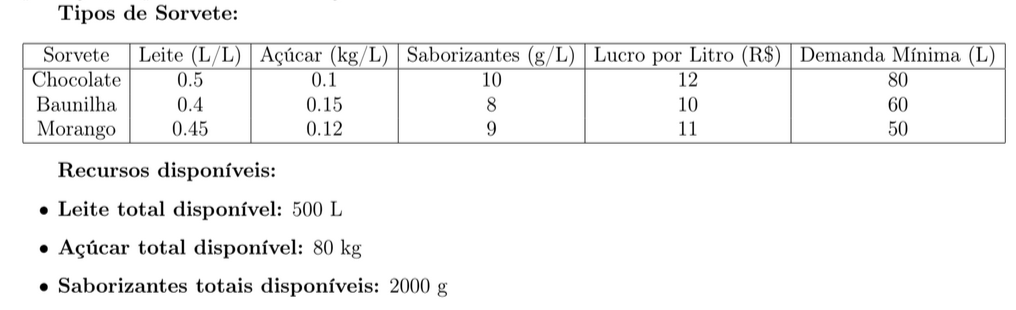
\includegraphics[scale=0.4]{image.png}

\textbf{Programa linear:}

\begin{equation}
    \text{max } 12x_c + 10x_b + 11x_m
\end{equation}

\begin{align}
    \text{s.a:} \nonumber \\
    0.5x_c + 0.4x_b + 0.45x_m &\leq 500 \\
    0.1x_c + 0.15x_b + 0.12x_m &\leq 80 \\
    10x_c + 8x_b + 9x_m &\leq 2000 \\
    x_c &\geq 80 \\
    x_b &\geq 60 \\
    x_m &\geq 50 \\
    %x_i &\geq 0, \text{ para } i \in \{c, b, m\} \\
    x_c, x_b, x_m &\in \mathbb{Q}^+
\end{align}

\textbf{Programa linear primal:}

\begin{equation}
    \text{min } -12x_c - 10x_b - 11x_m
\end{equation}

\begin{align}
    \text{s.a:} \nonumber \\
    -0.5x_c - 0.4x_b - 0.45x_m &\geq -500 \\
    -0.1x_c - 0.15x_b - 0.12x_m &\geq -80 \\
    -10x_c - 8x_b - 9x_m &\geq -2000 \\
    x_c &\geq 80 \\
    x_b &\geq 60 \\
    x_m &\geq 50 \\
    %x_i &\geq 0, \text{ para } i \in \{c, b, m\} \\
    x_c, x_b, x_m &\in \mathbb{Q}^+
\end{align}

\textbf{(b) Apresente o programa dual do entregue no item anterior. Proponha uma interpretação para as variáveis
duais.}

\textbf{Programa linear dual:}

\vspace{0.5cm}

\begin{equation}
    \text{max } -500y_l - 80y_a - 2000y_s +80y_c + 60y_b + 50y_m
\end{equation}

\begin{align}
    \text{s.a:} \nonumber \\
    -0.5y_l - 0.1y_a - 10y_s + y_c &\leq -12 \\
    -0.4y_l - 0.15y_a - 8y_s + y_b &\leq -10 \\
    -0.45y_l - 0.12y_a - 9y_s + y_m &\leq -11 \\
    y_l, y_a, y_s, y_c, y_b, y_m &\in \mathbb{Q}^+
    %x_i &\geq 0, \text{ para } i \in \{c, b, m\} \\
\end{align}

\textbf{Interpretação das variáveis duais:}

\begin{itemize}
    \item $y_l$: custo do leite por litro.
    \item $y_a$: custo do açúcar por litro.
    \item $y_s$: custo do saborizante por litro.
    \item $y_c$: custo do sorvete de chocolate por litro.
    \item $y_b$: custo do sorvete de baunilha por litro.
    \item $y_m$: custo do sorvete de morango por litro.
\end{itemize}

\vspace{0.5cm}

\textbf{(c) Apresente uma solução viável mas não ótima do primal e, usando folgas completares, mostre como
deduzir que tal solução não é ótima. (e) Explique o passo a passo.}

\vspace{0.5cm}

Sejam $x_c = 80$, $x_b = 60$, $x_m = 50$. Substituindo os valores nas restrições do primal, obtemos:

\begin{align*}
        -0.5x_c - 0.4x_b - 0.45x_m  = -86.5 > -500 \text{ (}y_l = 0\text{)} \\
        -0.1x_c - 0.15x_b - 0.12x_m  = -23 > -80 \text{ (}y_a = 0\text{)} \\
        -10x_c - 8x_b - 9x_m  = -1730 > -2000 \text{ (}y_s = 0\text{)} \\
    x_c = 80 \text{ (}y_c \geq 0\text{)} \\
    x_b = 60 \text{ (}y_b \geq 0\text{)} \\
    x_m = 50 \text{ (}y_m \geq 0\text{)}
\end{align*}

Analisamos as restrições duais:

\begin{align*}
    -0.5y_l - 0.1y_a - 10y_s + y_c = y_c &= -12 \\
    -0.4y_l - 0.15y_a - 8y_s + y_b = y_b &= -10 \\
    -0.45y_l - 0.12y_a - 9y_s + y_m = y_m &= -11 \\
\end{align*}

Como $y_c, y_b, y_m < 0$, a solução não é ótima.

\end{document}
